%=========================================================================
% (c) Michal Bidlo, Bohuslav Křena, 2008


\chapter{Úvod}

\chapter{Forenzní analýza digitálních dat} %???
Forenzní analýza digitálních dat je věda identifikující, zachovávající, obnovující, analyzující a předávající fakta ohledně digitálních důkazů nalezených v počítačích nebo digitálních úložištích mediálních zařízení.
Nezabývá se tedy pouze počítači, ale také ostatními digitálními technologiemi včetně mobilních telefonů a tabletů, mobilních sítí, internetového bankovnictví, datových médií apod. Pod výše uvedenými aktivitami se skrývá \cite{whatIsDigFor}:

\begin{itemize}
\item Identifikace - Jedná se o první část celého procesu. Předtím, než je cokoliv zkoumáno a analyzováno, je důležité identifikovat, kde jsou data uložena. Typicky jsou uložena na diskových jednotkách, serverech, flash klíčenkách, síťových zařízeních.

\item Zachování - Důležitá je ochrana důkazů, tzn. pro sběr a analýzu informací je potřeba zachovat původní data, musí se zabránit jejich změně a ztrátě. Bez integrity je důkazní materiál nepoužitelný.

\item Obnovení - Součástí procesu je i obnova dat, která může zahrnovat obnovu smazaných dat procesy operačního systému, úmyslně smazané soubory, soubory chráněné heslem a také poškozené soubory.

\item Analýza - Jedná se o hlavní část vyšetřování. Cílem je shromáždit co nejvíce relevantních artefaktů.

\item Předání - Po analýze jsou artefakty důkladně zdokumentovány a odevzdány například ve formě protokolu.
\end{itemize}

\noindent Vyšetřování digitálních forenzních dat obvykle zahrnuje vytvoření a prozkoumání obrazu disku. Obraz disku je kopie celého disku nebo jeho části bit po bitu. Obraz je statický snímek, který může být analyzován za účelem odhalení nebo stanovení událostí ohledně incidentů a být tak použitý jako důkaz v soudní síni. Analýza je prováděna na kopii pro zachování integrity originálu.

Vyšetřovatel zanalyzuje obraz pomocí snímacích technik, aby získal relevantní data z disku. Forenzní obraz obsahuje soubory z disku, ale také nealokovaný prostor a tzv. \texttt{slack space}. Slack space je pozůstatek diskového prostoru, který byl alokován pro nějaký počítačový soubor a ten všechen prostor nepotřebuje. Právě v těchto prostorech mohou být nalezeny relevantní informace jako například smazané soubory, či jejich fragmenty. \cite{forensicImages}

\section{Formáty digitálních forenzních dat}
Typů digitálních forenzních dat existuje spousta. Každý typ takových dat může být reprezentován jiným formátem. Tato sekce čerpá informace převážně z \cite{forensicswikiForensicFF}.

Mnoho forenzních počítačových programů používají své vlastní formáty pro uložení informace. Můžeme je rozdělit na nezávislé (anglicky \texttt{Independent File Formats}) a programově-specifické formáty (anglicky \texttt{Program-Specific File Formats}).

\begin{itemize}
\item Independent File Formats - Tyto formáty byly vyvinuty nezávisle na konkrétním forenzním programu. Patří mezi ně \texttt{AFF}, \texttt{AFF4}, \texttt{gfzip}, \texttt{Raw Image Format}.

\item Program-Specific File Formats - Byly vyvinuty pro použití specifickými forenzními programy. Většinou každý takový formát je unikátní a proto je pro přečtení potřeba unikátního nástroje.
Zástupci jsou například \texttt{Encase image file format}, \texttt{ProDiscover image file format}, \texttt{IXimager file formats}.
\end{itemize}

\noindent Vyznamným zástupcem je systém AFF4, který bude popsán detailněji.

\section{AFF4}
Celým názvem \texttt{The Advanced Forensics File Format 4} se jedná o open source formát pro ukládání digitálních důkazů a dat. Jeho výhodami jsou správa metadat a možnost komprese. Tato sekce čerpá převážně z\cite{aff4}. Je založen na objektově orientované architektuře. Veškerá množina známých objektů je označována jako \texttt{AFF4 universe}. Takový prostor je definovaný jako nekonečný, protože AFF4 je navržen pro škálování obrovského množství důkazního materiálu. Všechny objekty jsou adresovatelné jejich jménem, které je v rámci AFF4 universe unikátní.

\vspace{0.5cm}

\noindent Příkladem jména nějakého AFF4 objektu může být:

\texttt{urn:aff4:f3eba626-505a-4730-8216-1987853bc4d2}

\noindent Jedná se o standardní URN notaci, URN je unikátní.

\vspace{0.5cm}

\noindent AFF4 universe používá RDF notaci pro specifikaci atributů objektů. V nejjednodušší podobě je RDF množina tvrzení o objektu ve formátu:

\texttt{Subject   Attribute   Value}

\vspace{0.5cm}

\noindent Příklad:

\noindent \texttt{******** Object urn:aff4:f3eba626-505a-4730-8216-1987853bc4d2 ***********}\\
\texttt{aff4:stored = urn:aff4:4bdbf8bc-d8a5-40cb-9af0-fd7e4d0e2c9e}\\
\texttt{aff4:type = image}\\
\texttt{aff4:interface = stream}\\
\texttt{aff4:timestamp = 0x49E9DEC3}\\
\texttt{aff4:chunk\_size = 32k}\\
\texttt{aff4:compression = 8}\\
\texttt{aff4:chunks\_in\_segment = 2048}\\
\texttt{aff4:size = 10485760}\\

\noindent Příklad ukazuje, že objekt má tyto atributy a hodnoty. Nazýváme je relace nebo fakta. Celý AFF4 universe je sestavený z takových faktů.

\noindent AFF4 objekty existují, protože dělají něco užitečného, což závisí na rozhraní, které představují. Aktuálně existuje několik rozhraní, nejvýznamnější jsou \texttt{Volume} a \texttt{Stream}. Rozhraní objektu je fakt o objektu, který nalezneme v atributu \texttt{aff4:interface}.

\subsection{Rozhraní Volume}
Rozhraní Volume definujeme jako mechanismus ukládání, který dokáže uložit segment (bit binárních dat) pod nějaké jméno a získat jej podle tohoto jména. Aktuálně existují dvě implementace: \texttt{Directory} a \texttt{ZipFile}.

\begin{itemize}
\item \texttt{Directory Volume} - Tato implementace ukládá segmenty jako soubory uvnitř běžného adresáře v souborovém systému. Hodí se zejména, pokud potřebujeme uložit obraz na souborový systém FAT, přičemž velikost segmentu je malá a nenarazíme tak na omezení velikosti souboru. Je také možné založit adresář na nějaké http adrese, což nám umožní používat obraz přímo z webu.

\item \texttt{ZipFile Volume} - Jak napovídá název, tato implementace ukládá segmenty uvnitř zip archivu. Malé soubory lze tak bez problémů otevřít obyčejným průzkumníkem (windows explorer) a data extrahovat. Zase je možné zapsat zip archiv přímo na HTTP server a používat obraz přímo ze serveru.
\end{itemize}

\noindent Je možnost převádět mezi oběma formáty z jednoho na druhý, extrahovat zip archiv do adresáře a vytvoření Directory volume.

\subsection{Rozhraní Stream}
Streamy jsou základním rozhraním pro ukládání dat obrazu. Stream obsahuje metody typu \texttt{read}, \texttt{seek}, \texttt{tell} a \texttt{close}. Podporuje ještě \texttt{write}, ale ne k modifikaci obrazu, nýbrž k jeho vytvoření. Pokud nějaký AFF4 objektu podporuje rozhraní stream, lze provést náhodné čtení jeho dat. Existuje několik specifických implementací rozhraní stream, některými z nich jsou:

\begin{itemize}
\item \texttt{FileBackedObjects} - Stream, který ukládá data v souboru v souborovém systému, jehož pozice je určena URN souboru.

\item \texttt{HTTPObject} - Pozice souboru je udána pomocí URL. Objekt lze ukládat a číst z HTTP serveru. Implementace umožňuje přečíst určité rozmezí bajtů, režie síťového provozu mezi klientem a serverem je minimální. Je možné vyšetřit vzdálený obraz přes http bez potřeby celé kopie obrazu. Server musí být samozřejmě zabezpečen, ale to už AFF neřeší.

\item \texttt{Segments} - Segmenty jsou komponenty uloženy přímo ve \texttt{Volume}. Volume je zjednodušeně řečeno objekt uchovávající segmenty. Segmenty by měly být použity pro malé streamy, protože prohledávat v komprimovaných segmentech může být drahá operace. Segmenty jsou užitečné, pokud potřebujeme vytvořit logický obraz nějaké podmnožiny souborového systému (pouze některé soubory) a ne forenzní obraz celkového systému.

\item \texttt{Image streams} - Tyto streamy jsou opakem segmentů. Pro velké obrazy nemůžeme použít segmenty, protože by nebyly zkomprimovány efektivně. Image stream ukládá obraz v tzv. \texttt{chunks}.
\end{itemize}

\chapter{Úložiště pro rozsáhlá strukturovaná i nestrukturovaná data}
V této kapitole budou vysvětleny termíny Big data, distribuované databáze a NoSQL databáze, včetně jejich vlastností, výhod a nevýhod.

\section{Big data}
Definicí pro frázi Big data existuje několik. Jedná se o termín použitý na soubory dat, které jsou příliš komplexní z hlediska velikosti a různorodosti, a které je nemožné zpracovávat běžně používanými přístupy a softwarovými nástroji v rozumném čase.

Objem takových dat rychle roste. Vyskytují se v mnoha odvětvích, například sběr informací o počasí, sociální sítě, energetické a telekomunikační společnosti, ekonomie a finančnictví, či data z kamer, měření z různých senzorů apod. Z toho plyne, že se jedná o data různorodých typů, mohou být strukturovaná i nestrukturovaná. Proto je potřeba existence různých technologií pro jejich uložení, zpracování i zobrazení.

\begin{figure}[!h]
  \centering
  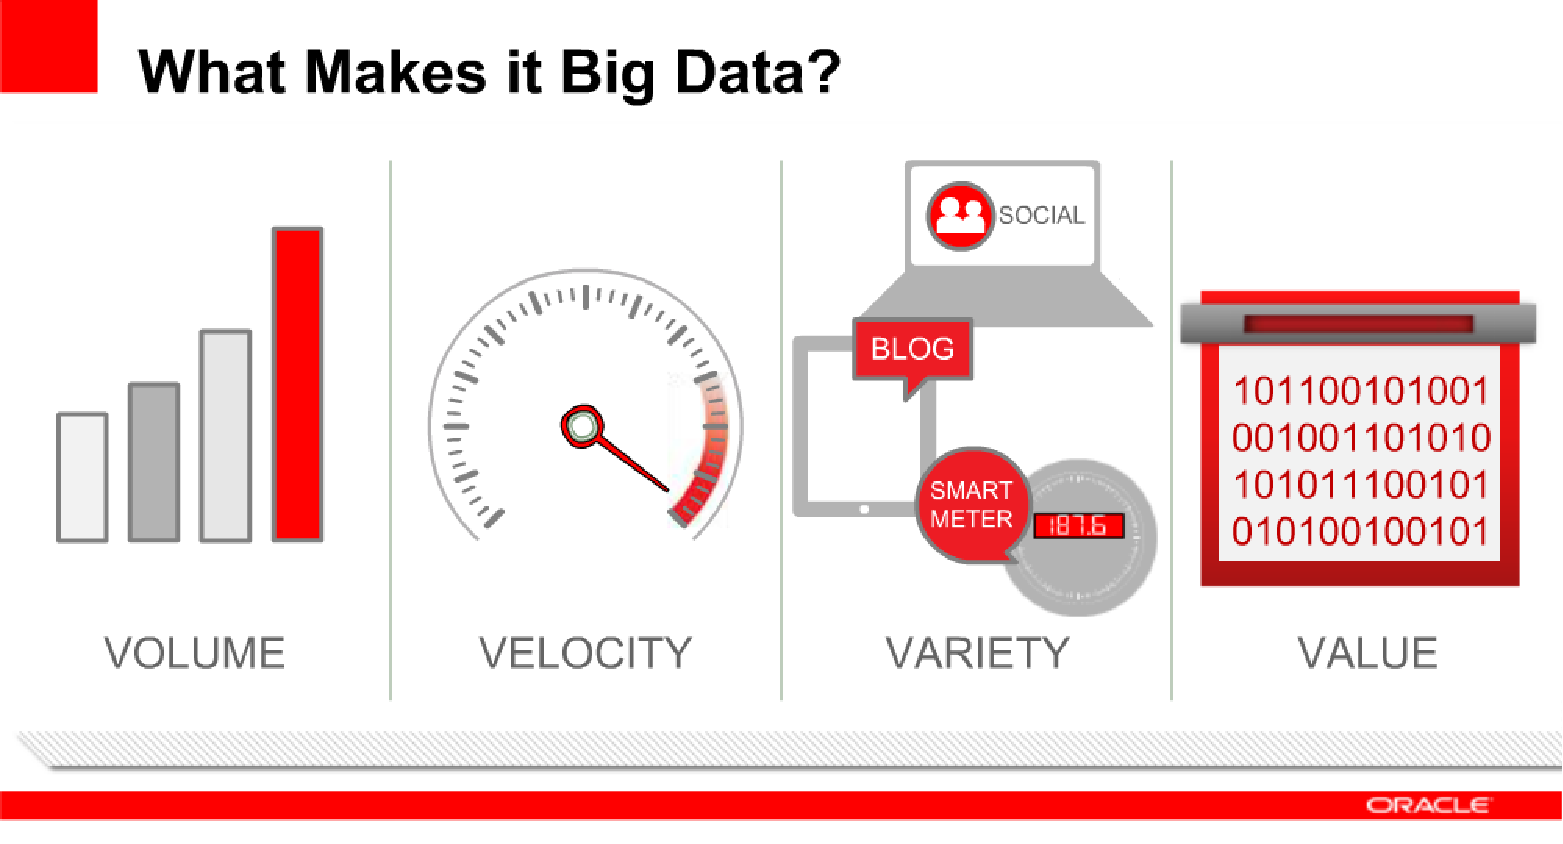
\includegraphics[width=12.5cm]{template-fig/what_makes_data_big_data.pdf}
  \caption{Definice Big data podle Oracle. \cite{johanBigData}}
  \label{FIG_BigData}
\end{figure}

\noindent Big data je často definováno jako 4V z anglických slov Volume, Velocity, Variety a Value. \cite{oracleBigData}

\begin{itemize}
\item Volume – značí množství nebo velikost dat. Big data vyžaduje zpracování vysokých objemů dat neznámých hodnot, například síťový provoz, data sesbírána ze senzorů apod.

\item Velocity – vyjadřuje rychlost z hlediska vzniku dat a potřeby jejich analýzy, některá vyžadují zpracování v reálném čase. Nejdůležitější data se zapisují přímo do paměti, a ne na disk, z důvodu co nejrychlejšího zpracování.

\item Variety – znamená různorodost typů. Jedná se především o nestrukturovaná data, například text, audio, video, data o geografické poloze a další. Jsou na ně kladeny velmi podobné požadavky jako na data strukturovaná – sumarizace, monitorování, důvěrnost. \cite{oracleBigData}

\item Value – data mají vlastní hodnotu, která musí být analyzována a zjištěna. Nejedná se o jednoduchý proces, je stále potřeba nových metod a technik zpracování.
\end{itemize}

\begin{figure}[!h]
  \centering
  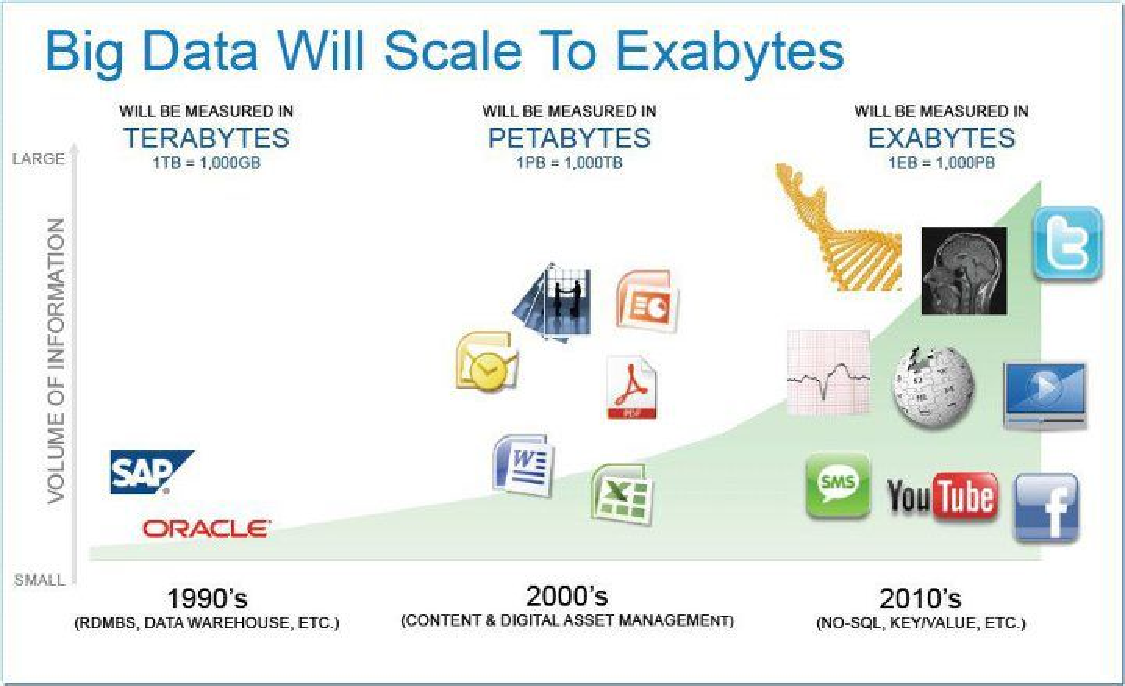
\includegraphics[width=15cm]{template-fig/big_data_exabytes.pdf}
  \caption{S novými technologiemi se masivně zvyšuje růst dat a přibývají nové typy. \cite{rajeshBigData}}
  \label{FIG_BigDataExabytes}
\end{figure}

\noindent Tato práce se zabývá Big daty hlavně typu – PCAP soubory, logy ze síťových zařízení a komunikací. Možnosti uložení Big data budou popsány v následujících podkapitolách.

\section{Distribuované databáze}
Distribuovaná databáze se skládá z většího počtu samostatných databází, které mohou být geograficky rozmístěny na jiných pozicích. Jednotlivé uzly spolu komunikují přes počítačovou síť. Každý uzel je sám o sobě databázový systém. DSŘBD neboli systém řízení distribuované báze dat (anglicky Distributed Database Database Management System) zajišťuje, že se distribuovaná databáze uživatelům jeví jako jedna jediná databáze. Data jsou fyzicky uložena na různých pozicích. Mohou být spravována rozdílnými SŘBD nezávisle na ostatních pozicích. \cite{distributedDBMS}

Systém řízení distribuované báze dat je centralizovaný systém s těmito vlastnostmi 
\cite{distributedDBMS}:

\begin{itemize}
\item Umí vytvářet, získávat, upravovat a mazat distribuované databáze. Zajišťuje důvěrnost a integritu databází.

\item Periodicky synchronizuje databázi a poskytuje mechanismy přístupu tak, aby se databáze uživatelům jevila transparentní.

\item Zajišťuje, že změna dat v kterémkoliv uzlu se promítne i v ostatních uzlech.

\item Je využíván v aplikacích, kde se předpokládá zpracování velkých objemů dat, ke kterým přistupuje současně mnoho uživatelů.
\end{itemize}

\begin{figure}[!h]
  \centering
  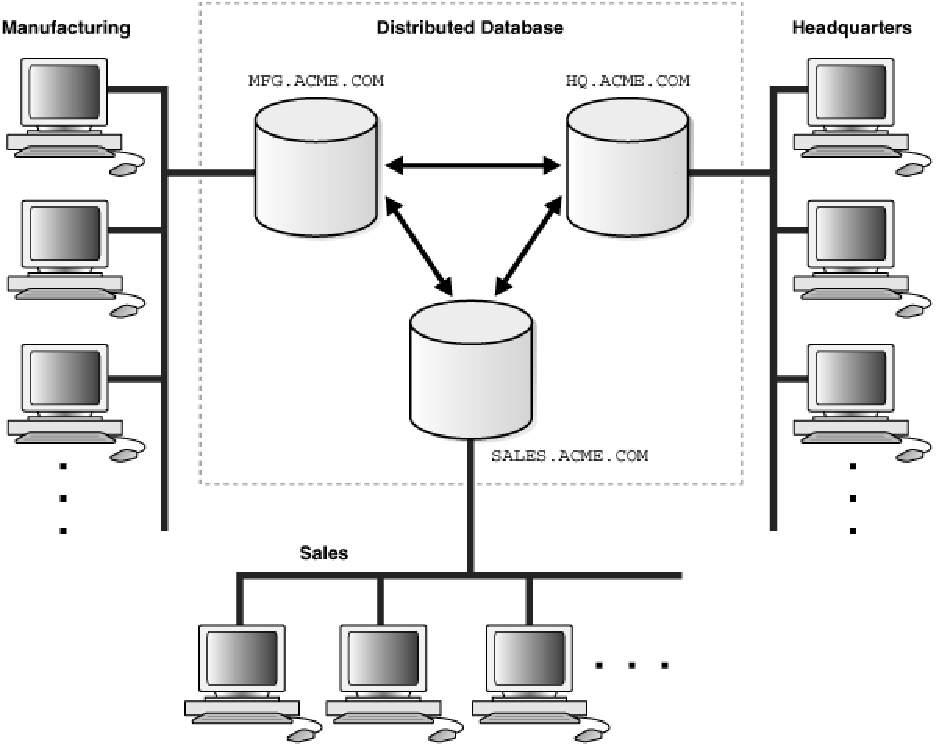
\includegraphics[width=15cm]{template-fig/Distributed_database.pdf}
  \caption{Schéma distribuované databáze a současný přístup více zařízení k ní. \cite{distributedDBMSPic}}
  \label{FIG_DistrDB}
\end{figure}

Výhody
\begin{itemize}
\item Rozšiřitelnost – pokud je potřeba databázový systém rozšířit do nových míst nebo přidat další uzly, stačí přidat nový(é) počítač(e) a lokální data v nové pozici, a nakonec je připojit k distribuovanému systému, bez jakéhokoliv přerušení funkcionality. Podobný postup je při odebrání uzlu.

\item Spolehlivost – když nějaký z připojených uzlů selže, nepřestane distribuovaná databáze fungovat, sníží se maximálně výkon.

\item Ochrana (záloha) dat – při zničení jednoho uzlu a smazání dat z něj, mohou být stejná data zálohována i na jiných uzlech.

\item Výkonnost – pokud jsou data efektivně distribuována, může být uživatelův požadavek uspokojen rychleji. Transakce mohou být také distribuované a provedeny rychleji. 
\end{itemize}

Nevýhody
\begin{itemize}
\item Integrita dat – data musí být průběžně synchronizována na více uzlech, aby na stejné dotazy nebyly z různých uzlů vraceny rozdílné odpovědi.

\item Komunikační režie – i zdánlivě jednoduchá operace může vyžadovat spoustu zbytečné komunikace.

\item Cena – DSŘDB vyžaduje drahý a složitý software ke koordinaci uzlu a zajištění transparentnosti. \cite{distributedDBMS}

\item Mezi další patří – složitost, zabezpečení, řízení souběžného přístupu k datům.
\end{itemize}

\begin{figure}[!h]
  \centering
  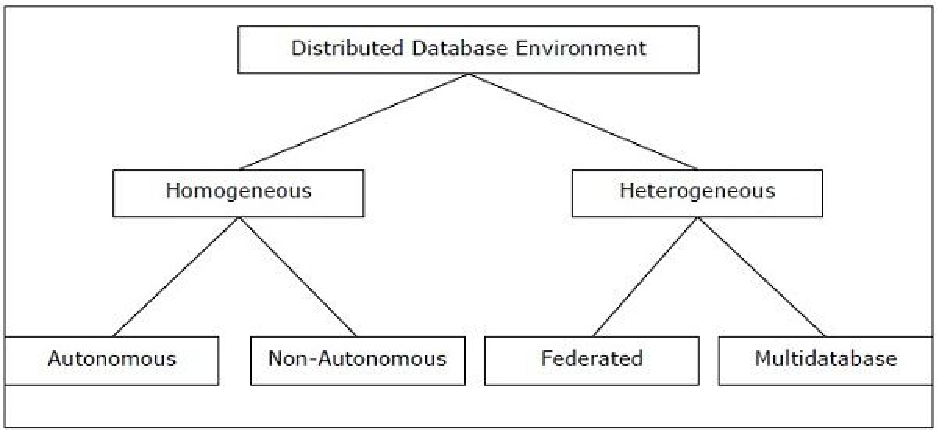
\includegraphics[width=15cm]{template-fig/distributed_database_environments.pdf}
  \caption{Distribuované databáze můžeme rozdělit na homogenní a heterogenní, a tyto ještě dále dělit. \cite{distributedDBMS}}
  \label{FIG_DivDistrDB}
\end{figure}

\noindent Homogenní – všechny uzly používají identické SŘBD a operační systémy. Uzly mají informace o ostatních uzlech a spolupracují při zpracování uživatelských požadavků. Homogenní distribuovaná databáze se navenek jeví uživateli jako jeden systém. Je jednodušší jej navrhnout a spravovat.

Heterogenní – uzly mohou mít rozdílné operační systémy a SŘBD, které nejsou kompatibilní. Mohou také využívat rozdílná schémata (relační, objektově orientované, hierarchické, \ldots). Rozdílnost schématu je hlavním problémem při zpracování dotazu a transakcí. Kvůli tomu je také složité dotazování. \cite{wikiDBMS}

Architekturami distribuovaných databází jsou centrální architektura, klient-server, peer-to-peer, multi-databázová architektura.


\section{NoSQL, disky, úložiště}

\chapter{Návrh distribuovaného úložiště}
\section{Přístup k datům}
\subsection{Sekvenční, náhodný}
\subsection{Dotazování}
\subsection{Big data přístupy}
\section{Architektura}
\section{Aplikační rozhraní}
\section{Technologie}
\subsection{Docker}
\subsection{HDFS, Hadoop, Spark}
\subsection{Cassandra / MongoDB}
\subsection{Zookeeper}
\subsection{MQ broker}

\chapter{Implementace}
\section{Rozšiřitelnost, znuvupoužitelnost}

\chapter{Testování}
\section{Výkon}

\chapter{Závěr}

%=========================================================================
